% !TEX TS-program = Xelatex
% !TEX encoding = UTF-8 Unicode

\documentclass[UTF8]{ctexart}
\usepackage{amsmath}
\usepackage{geometry}
\usepackage{graphicx}
\usepackage{figsize}
\usepackage{ gensymb }
\geometry{left=0.7in,right=0.7in,bottom=0.7in,top=0.7in}

\title{预科实验三:测量元件的伏安特性}
\author{朱寅杰 1600017721}
\date{2017年10月13日}

\begin{document}

\maketitle

\section{实验数据}

\subsection{未知电阻的测量}

两个未知电阻的阻值用万用表粗测,分别是$R_1=46.9$\ohm ,$R_2=1.005$k\ohm 。表笔短路时未测得有电阻。

% \newline
测量使用指针式电压表和电流表。根据粗测结果,对阻值较小的$R_1$将电流表外接,对阻值较大的$R_2$将电流表内接,记录得不同电压下通过电阻的电流如下:

% \newline

\begin{tabular*}{0.95\textwidth}{@{\extracolsep{\fill}}c|c c|c c}
\hline
序号	&$U_1$/V	&$I_1$/mA	&$U_2$/V	&$I_2$/mA\\
\hline
1	&0.079	&2.04	&0.390	&0.368
\\
2	&0.117	&2.95	&0.758	&0.744
\\
3	&0.160	&4.04	&1.044	&1.016
\\
4	&0.213	&5.32	&1.442	&1.382
\\
5	&0.268	&6.59	&1.646	&1.606
\\
6	&0.372	&9.19	&2.194	&2.136
\\
7	&0.558	&13.69	&2.876	&2.796
\\
\hline

\end{tabular*}

% \newline
根据表中数据,作出$U_1-I_1$与$U_2-I_2$的图像,从图中分别分析出$U/I$的值。

\begin{figure}
\centering
\SetFigLayout{2}{1}
\subfigure[$R_1$的$I-U$伏安特性曲线。根据回归分析得到电阻为$R_1=\frac{1}{24.443\times10^{-3}\ohm^{-1}}=40.9\ohm$]{\includegraphics{R_1.ps}} \\
\subfigure[$R_2$的$I-U$伏安特性曲线。根据回归分析得到电阻为$R_2=\frac{1}{0.9734\times10^{-3}\ohm^{-1}}=1027\ohm$]{\includegraphics{R_2.ps}} \\
\end{figure}

% \newline
测量$R_1$时电流表外接,应对电压表的内阻进行修正。电表标称的内阻为200\ohm/V,测量时使用的是1.5V量程,对应的内阻为300\ohm 。修正下来以后得到的结果是47.4\ohm 。

% \newline
测量$R_2$时电流表外接,应对电流表的内阻进行修正。测量时使用的是3mA量程,对应的内阻为24.1\ohm 。修正下来以后是1003\ohm 。


\subsection{稳压二极管的伏安特性}

测量使用两台数字万用表分别测量二极管两端电压与通过的电流。在测量过程中切换过量程,电流档使用过$200\mu$A、2mA与20mA三档,电压档使用过2V与20V两档,因此表中的各个数据的有效位数会有差异。

测量数据见下表。电压档位的仪器允差为0.05\%+3个字,电流档位的仪器允差为0.5\%+4个字。

\begin{tabular*}{0.95\textwidth}{@{\extracolsep{\fill}}c c|c c}
\hline
电压$U$/V	&电流$I$/mA	&(续)电压$U$/V	&电流$I$/mA\\
\hline
-5.540	&-19.488	&(0)	&(0)
\\
-5.530	&-15.866	&0.4976	&0.00395
\\
-5.525	&-13.704	&0.5245	&0.00723
\\
-5.517	&-11.070	&0.5643	&0.01621
\\
-5.515	&-10.444	&0.6141	&0.04743
\\
-5.513	&-10.000	&0.6445	&0.09629
\\
-5.511	&-9.895	&0.6592	&0.13781
\\
-5.509	&-9.793	&0.6732	&0.19634
\\
-5.507	&-9.418	&0.6961	&0.3601
\\
-5.502	&-8.194	&0.7133	&0.5802
\\
-5.500	&-7.544	&0.7292	&0.9170
\\
-5.496	&-6.144	&0.7435	&1.3989
\\
-5.492	&-4.643	&0.7624	&2.485
\\
-5.487	&-3.231	&0.7883	&5.508
\\
-5.483	&-2.234	&0.7949	&6.752
\\
-5.479	&-1.4352	&0.8000	&7.954
\\
-5.476	&-0.9742	&0.8074	&10.060
\\
-5.472	&-0.5659	&	&
\\
-5.469	&-0.3666	&	&
\\
-5.462	&-0.2366	&	&
\\
-5.453	&-0.1808	&	&
\\
-5.419	&-0.1017	&	&
\\
-4.000	&-0.00195	&	&
\\
-2.789	&-0.00064	&	&
\\
\hline

\end{tabular*}

根据表中数据作出二极管的伏安特性曲线见下页图所示。

\begin{figure}
\centering
\SetFigLayout{2}{1}
\subfigure[稳压二极管的伏安特性]{\includegraphics{diode.ps}} \\
\subfigure[稳压段局部放大图。图中水平与垂直的误差线分别是由电表电压和电流档的基本误差估计的数据的不确定度。]{\includegraphics{10mA.ps}} \\
% \caption{稳压二极管的伏安特性曲线}\label{fig:1}
\end{figure}

从中可以计算出二极管在0.8V处的静态电阻为$R=U/I=0.8000$V$/7.954$mA$=100.6\ohm$,在-4.0V处的静态电阻为$R=U/I=(-4.000$V$)/(-1.95\mu$A$)=2.05$M\ohm  。这反映出二极管具有单向导电的特性。

还要求计算电流为-10mA处,二极管的动态电阻$R'=dU/dI$。我们将伏安曲线中稳压这一段放大看(见图(d)),并且将由电表允差算得的测量不确定度标注于图上。可以看出尽管数字电表电流档的允差约是电压档的十倍,但对于微商的计算来说,电压档误差对计算造成的困难远大于电流档。并且更让人郁闷的是,在测量时本来有意在电流快要达到10mA时多采几个数据点好算微商,当场粗粗一算觉得没啥问题,一作图才发现这几个数据点反倒成了大麻烦。整个稳压段一条直线仿佛被10mA附近这几个点割裂成了两段斜率相近但截距不同左右有些错开的直线,这样一来如果要求10mA处的斜率,那么取附近的不同的点算出来的微商就会相差非常大,而且看图上误差线的长度,这样求得的微商似乎甚至一位有效数字都没有。(也就是说我这几个数据可以说是白测了……)还是取远一些的点来算吧。取(-5.492V,-4.643mA)和(-5.530V,-15.866mA)这两个点,算出动态电阻为3.4\ohm ;取(5.525V, 13.704mA)和(5.496V, 6.144mA)计算得动态电阻为3.8\ohm ,因此我们做出估计说-10mA附近的动态电阻大概就在3~4\ohm 左右。这个数量级的动态电阻证明这个稳压二极管的稳压性能还是不错的。

至于为什么-10mA附近的曲线恰好有一个断层呢?当然你可以指着误差线说这完全在误差范围之内嘛,甚至可以在所有误差线范围内拉出一条直线来,所以这算不上什么大惊小怪的事情。但是这么整齐划一的各自往一边倒以至于把图线割成两层的偏差还是让人很奇怪。测量时为了调出这10mA附近的几个数据点,曾多次左右细调两个分压的滑动变阻器,难道说数字电表上微小数值变化的触发也有类似于鼓轮的空程差的效应?还是我在测这几个点的时候做了别的什么影响到电表或是元件的事情么?

\section{思考题}
\subsection{}
多用表的欧姆档的测量原理也可以看作是伏安法,使用不同档位时,加在元件上的分压不一样,对于二极管这样的非线性元件来说就会表现出不一样的电阻值。如果是线性电阻则不会发生这样的现象。

\subsection{}
在测量二极管时,由于数字万用表的电压档的内阻极其大(都在M\ohm  以上),而电流档的内阻相对不小(测量压降会有数十到数百mV),甚至与二极管的正向电阻可以比较,因此在测量二极管正向特性时电流表应该外接。

\subsection{}
从实验数据可以看出,修正电表误差后的电阻测量值(47.4\ohm 与1003\ohm )比起修正前(40.9\ohm 与1027\ohm )更接近于用万用表直接测量的电阻值(46.9\ohm 与1.005k\ohm ),证明修正电表带来的系统误差对于测量的结果是有不小的改善的。

\end{document}


